\PassOptionsToPackage{unicode}{hyperref}
\documentclass[
  ukrainian,
  14pt
]{extreport}
\usepackage{lmodern}
\usepackage{hyperref}
\makeatletter
\hypersetup{
    colorlinks=true,
    linkcolor=blue,
    filecolor=magenta,
    urlcolor=cyan,
}
\makeatother
\usepackage{amssymb,amsmath,amsthm,url}
\usepackage[margin=2cm]{geometry}
\usepackage{longtable,booktabs}
\usepackage{etoolbox}
\usepackage{titling}
\usepackage{graphicx}
\usepackage{float}
\usepackage[dvipsnames]{xcolor}
\usepackage[ukrainian]{babel}
\usepackage{setspace}
\usepackage{xcolor}
\usepackage{multirow}
\usepackage{comment}
\usepackage{booktabs}
\usepackage{tikz}
\setcounter{secnumdepth}{-1} 
\usepackage{unicode-math}
  \defaultfontfeatures{Scale=MatchLowercase}
  \defaultfontfeatures[\rmfamily]{Ligatures=TeX,Scale=1}
  \setmainfont[]{Times New Roman}
  \setsansfont[]{Arial}
  \setmonofont[]{Consolas}
  \makeatother
\usepackage[labelsep=period]{caption}
\usepackage{subcaption}

\author{}
\title{\Huge Лабораторна робота №2 \\\Large Дослідження ВАХ діодів}
\date{}
             
\begin{document}
\begin{titlepage} 
	\newcommand{\HRule}{\rule{\linewidth}{0.5mm}} 
	
	\center 
	
	\textsc{\Large МІНІСТЕРСТВО ОСВІТИ І НАУКИ УКРАЇНИ\\ \Large КИЇВСЬКИЙ НАЦІОНАЛЬНИЙ УНІВЕРСИТЕТ ІМЕНІ ТАРАСА ШЕВЧЕНКА}\\[1.5cm] 

	
	\HRule\\[0.4cm]
	
	{\huge \bfseries  Лабораторна робота №2 \\\Large \bfseries Моделювання пасивних RC фільтрів
    }\\[0.4cm]
	
	\HRule\\[1.5cm]

	
	

	{\large\textit{Автор}}\\
	\large Столяров Андрій Дмитрович, \\\large група 5-А, Фізичний Факультет 
	
	
	\vfill\vfill\vfill 
	\vfill
	{\normalsize Київ, \today} 
\end{titlepage}
\tableofcontents
\clearpage
\section{Вступ}
В даній роботі моделюють такі пасивні RC
фільтри: ФНЧ, ФВЧ, смуговий та
загороджувальний. Робота виконувалась у програмі \textbf{Multisim14}.
\subsection{Мета}
Дослідити зміну параметрів прямокутних імпульсів та гармонічних сигналів при
проходженні через пасивні лінійні чотириполюсники, опанувати методи вимірювання
амплітудно-частотних та фазо-частотних характеристик пасивних RC-фільтрів та їх перехідних характеристик
\subsection{Методи дослідження}
Метод співставлення, тобто одночасного спостереження вхідного та вихідного сигналів на екрані двоканального осцилографа із наступним вимірюванням і порівнянням
їх параметрів;
Метод фігур Лісажу, який полягає у спостереженні на екрані двоканального
осцилографа замкнених кривих, які є результатом накладання двох коливань, що відбуваються у двох взаємно перпендикулярних напрямках (вхідний і вихідний сигнали
подаються на пластини горизонтального та вертикального відхилення осцилографа відповідно).
\section{Теоретичні відомості}
\textbf{Чотириполюсник} -- це електричне коло (ділянка електричного кола) з чотирма
полюсами, зажимами, клемами або іншими засобами приєднання до нього інших електричних кіл чи ділянок електричних кіл.

\textbf{Пасивний чотириполюсник} -- це такий чотириполюсник, який не здатний
збільшувати потужність вхідного сигналу за рахунок додавання енергії від якогось іншого джерела енергії (внутрішнього чи зовнішнього по відношенню до чотириполюсника).
Потужність, що виділяється в елементі кола, підключеного до виходу такого чотириполюсника, менша за потужність, що споживається від джерела сигналу, підключеного до
входу чотириполюсника.

\textbf{Активний чотириполюсник} дозволяє збільшувати потужність вихідного сигналу порівняно з потужністю вхідного сигналу за рахунок внутрішніх або зовнішніх
джерел енергії. Має містити активний елемент.

\textbf{Лінійний чотириполюсник} — це такий, для якого залежність між струмами,
що течуть крізь нього, та напругами на його зажимах є лінійною. Такі чотириполюсники
складаються з лінійних елементів.

\textbf{Лінійні елементи електричних кіл }— це такі елементи, параметри яких не залежать від величини струму, що протікає через них або від прикладеної до них напруги.
На виході лінійних чотириполюсників, на відміну від нелінійних, не можуть утворюватися гармоніки ( і т. д.) сигналу частоти , який подано на вхід.

\textbf{Нелінійний чотириполюсник} – це такий, який містить нелінійні елементи.
Для нього згадані залежності між струмами та напругами при деяких їх величинах
перестають бути лінійними, а на виході можуть з’являтися гармоніки частот вхідних
сигналів

\textbf{Пасивний фільтр} — це пасивний чотириполюсник, який містить реактивні
елементи (індуктивності, ємності), спад напруги на яких або струм через які залежить від частоти, і завдяки цьому здатен перетворювати спектр сигналу, поданого на його вхід, шляхом послаблення певних спектральних складових вхідного сигналу. Решта
спектральних складових вхідного сигналу проходить через такий пасивний лінійний чотириполюсник, тобто він працює як фільтр для певних спектральних складових сигналу.
Фільтри, побудовані на конденсаторах і резисторах, називають RC-фільтрами.

\section{Хід Роботи}
В роботі використано метод фігур Лісажу. Цей метод полягає у спостереженні на екрані двоканального осцилографа
замкнених кривих, які є результатом накладання двох коливань, що відбуваються
у двох взаємно перпендикулярних напрямках (вхідний і вихідний сигнали
подаються на пластини горизонтального та вертикального відхилення
осцилографа відповідно).

\subsection{Фільтр низьких частот}
\begin{figure}[H]
  \centering
  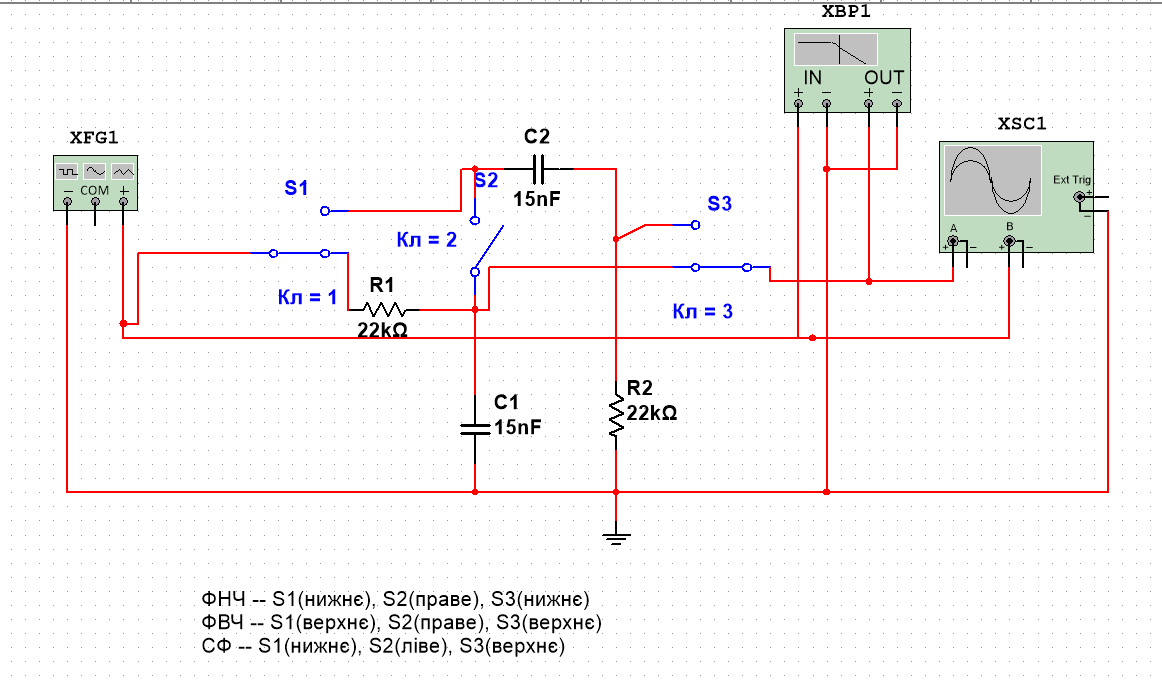
\includegraphics[width=.6\textwidth]{imgs/FNC-1.png}
  \caption{Схема ФНЧ}
\end{figure}
\begin{figure}[H]
  \centering
  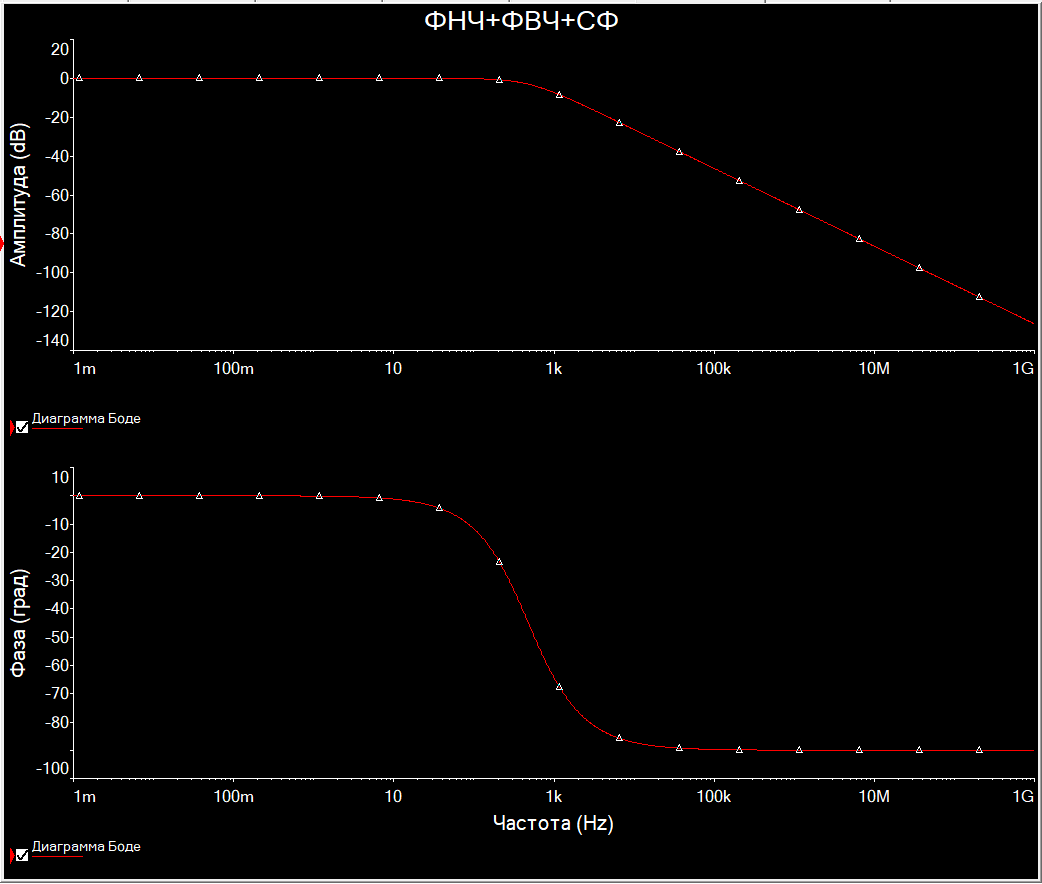
\includegraphics[width=.6\textwidth]{imgs/FNC-2.png}
  \caption{Частотна характеристика}
\end{figure}
\begin{figure}[H]
  \centering
  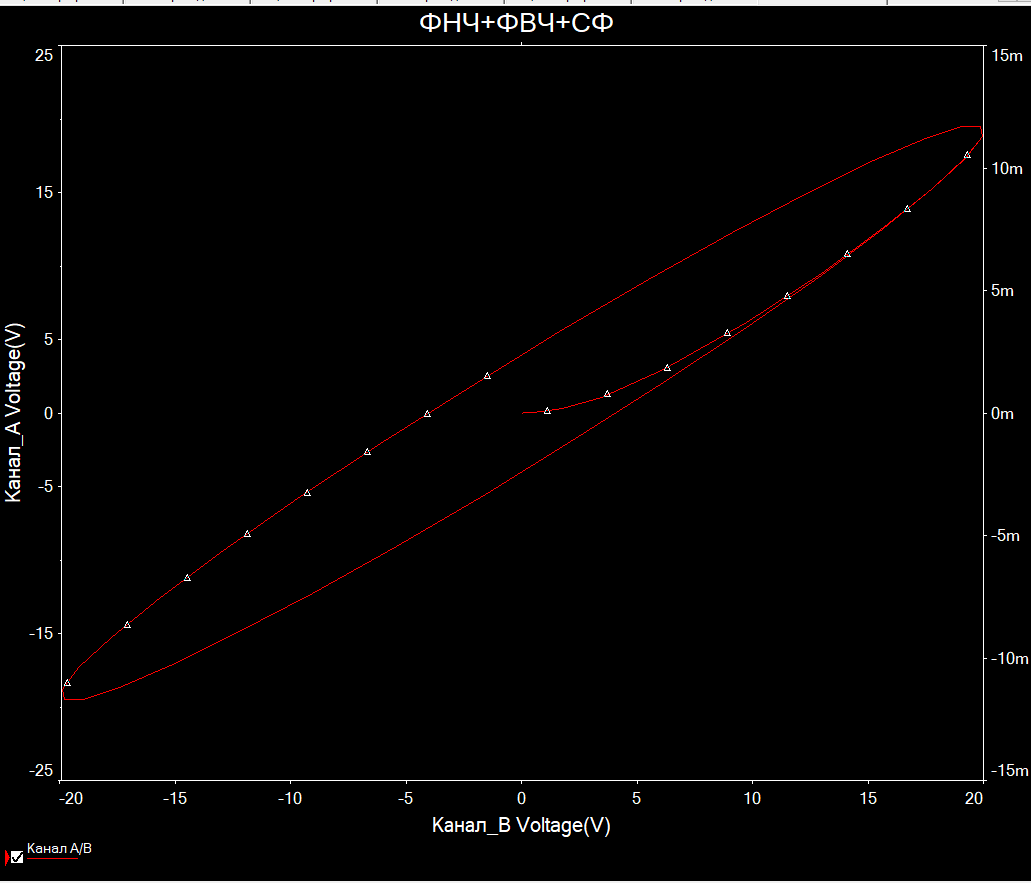
\includegraphics[width=.6\textwidth]{imgs/FNC-3.png}
  \caption{Фігура Лісажу}
\end{figure}
\begin{figure}[H]
  \centering
  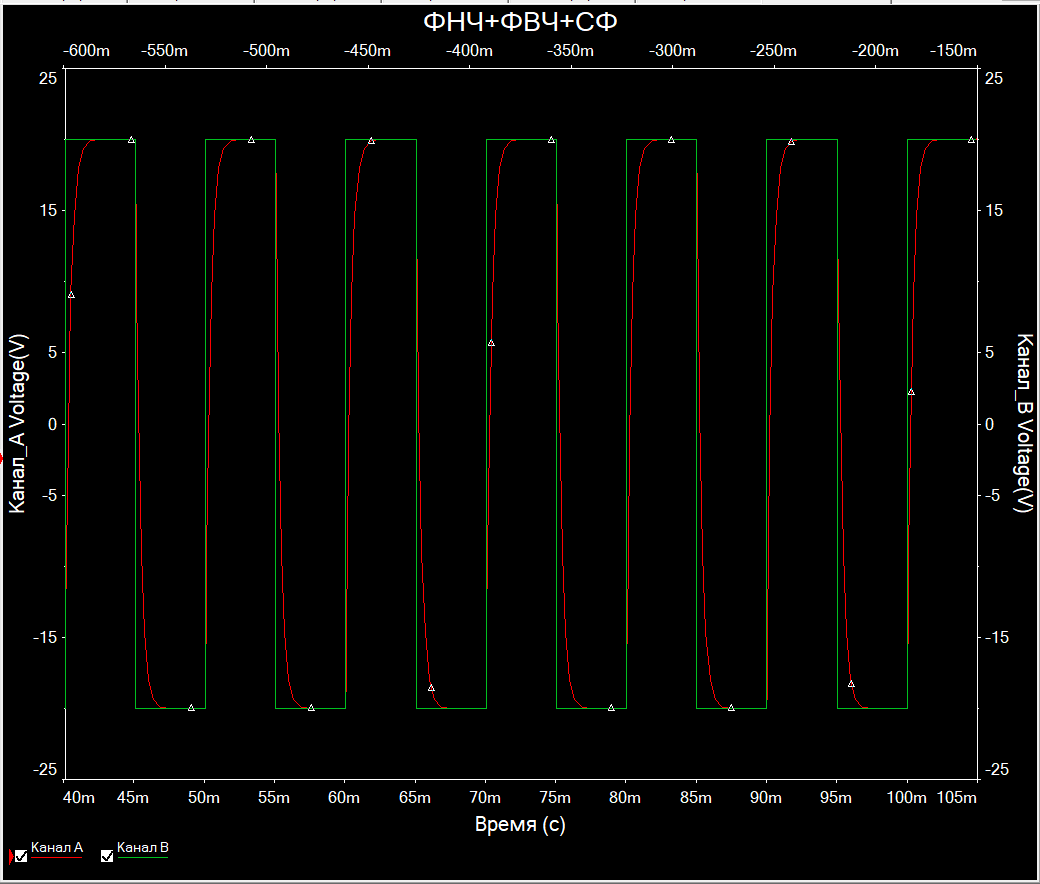
\includegraphics[width=.6\textwidth]{imgs/FNC-4.png}
  \caption{Реакція на дискретний сигнал}
\end{figure}

\subsection{Фільтр високих частот}
\begin{figure}[H]
  \centering
  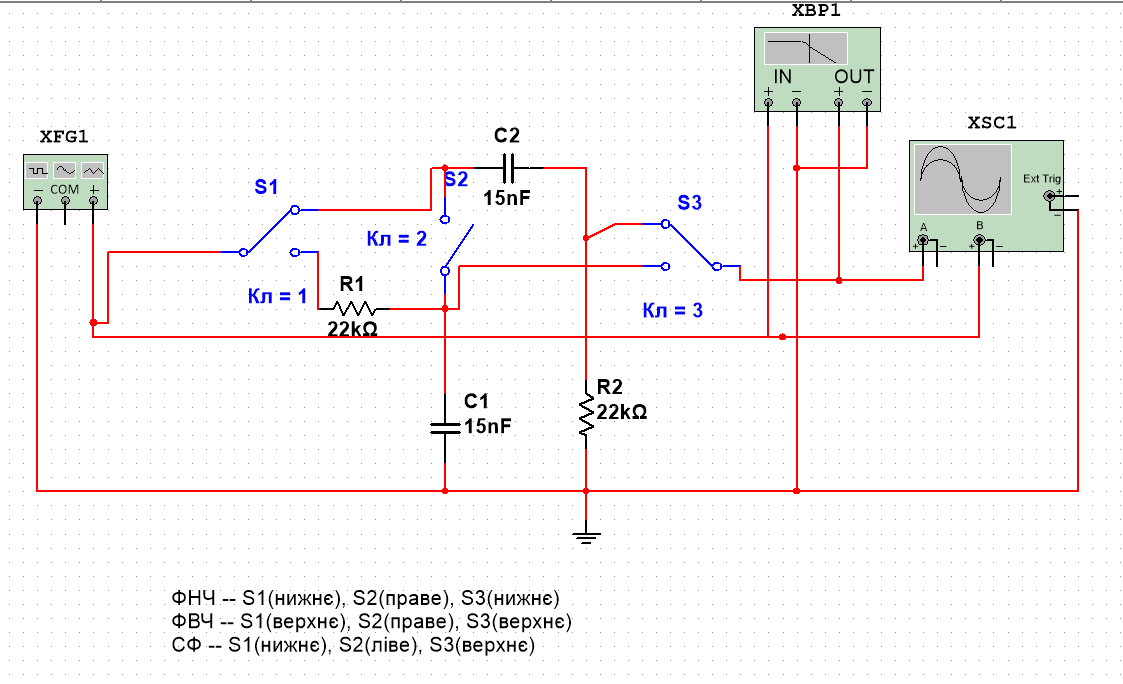
\includegraphics[width=.6\textwidth]{imgs/FVC-1.png}
  \caption{Схема ФВЧ}
\end{figure}
\begin{figure}[H]
  \centering
  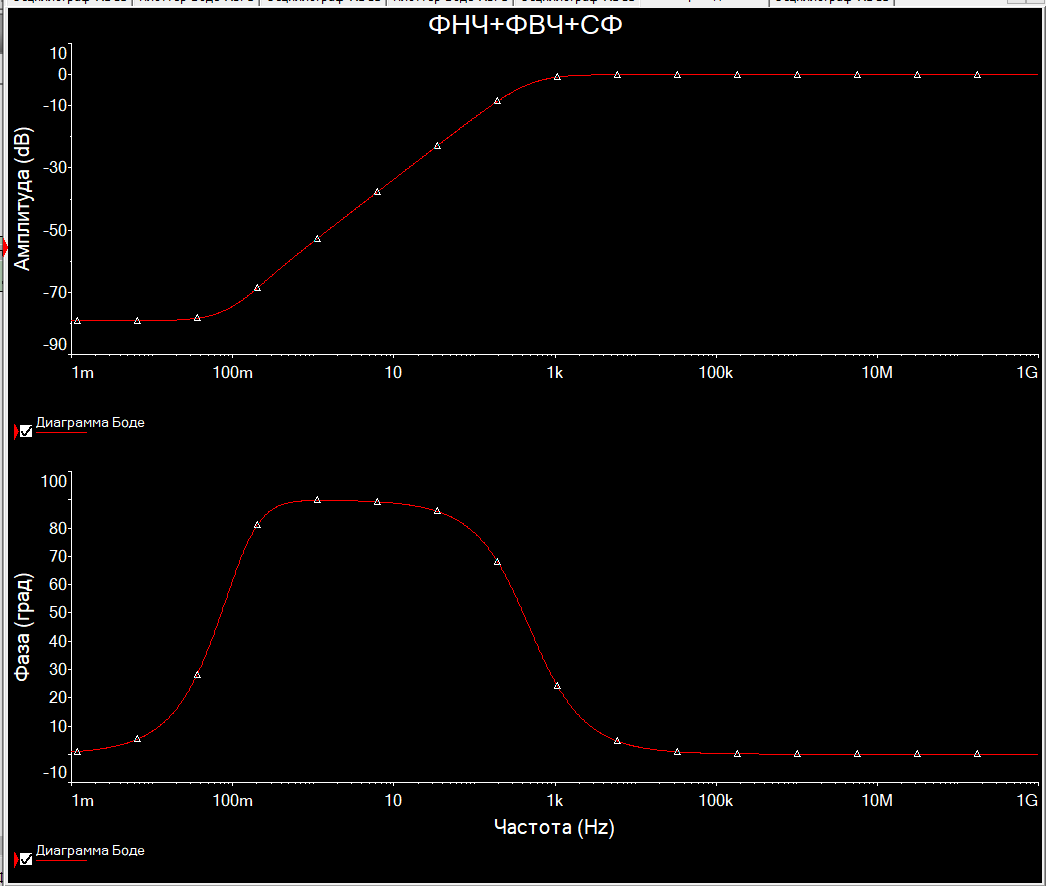
\includegraphics[width=.6\textwidth]{imgs/FVC-2.png}
  \caption{Частотна характеристика}
\end{figure}
\begin{figure}[H]
  \centering
  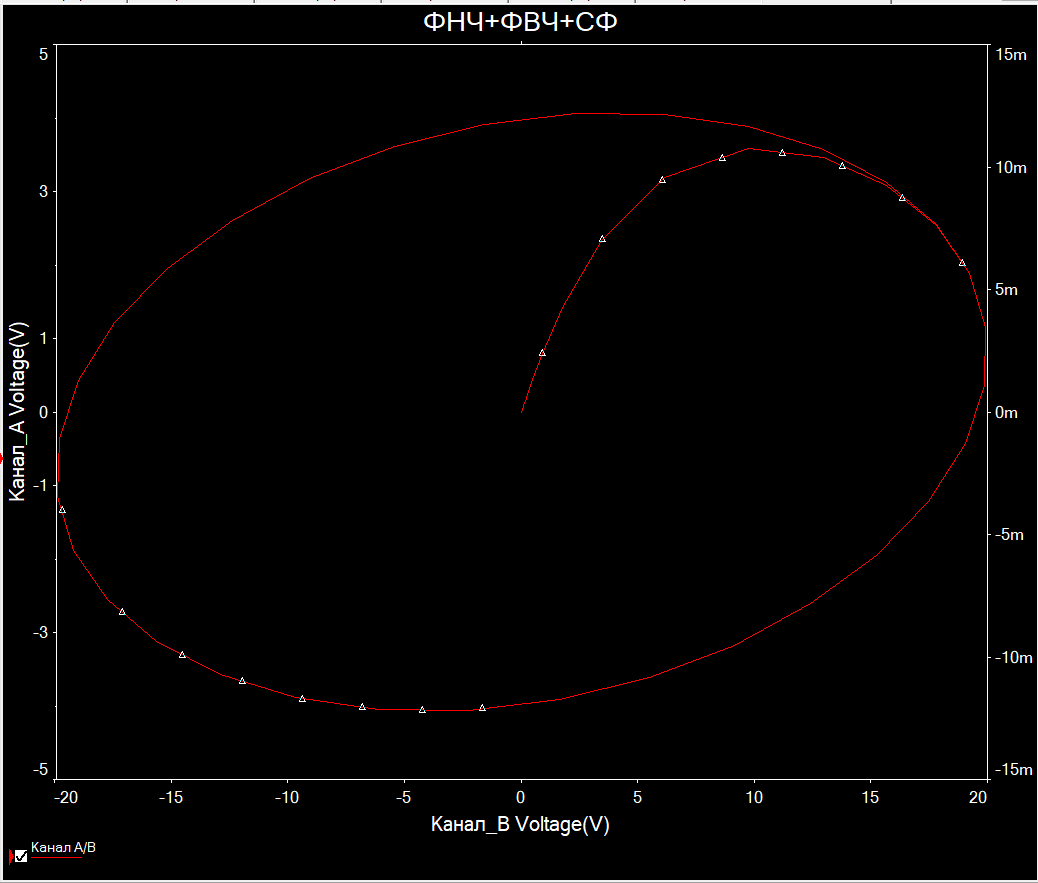
\includegraphics[width=.6\textwidth]{imgs/FVC-3.png}
  \caption{Фігура Лісажу}
\end{figure}
\begin{figure}[H]
  \centering
  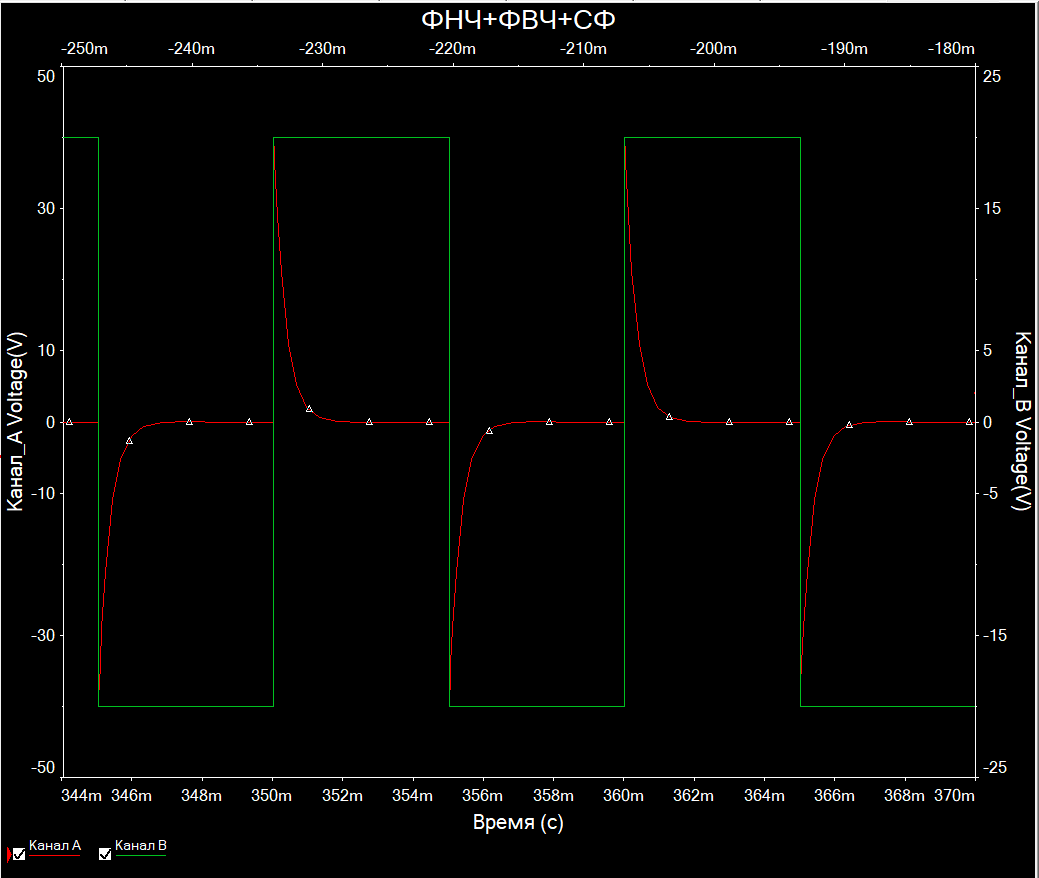
\includegraphics[width=.6\textwidth]{imgs/FVC-4.png}
  \caption{Реакція на дискретний сигнал}
\end{figure}

\subsection{Смуговий Фільтр}
\begin{figure}[H]
  \centering
  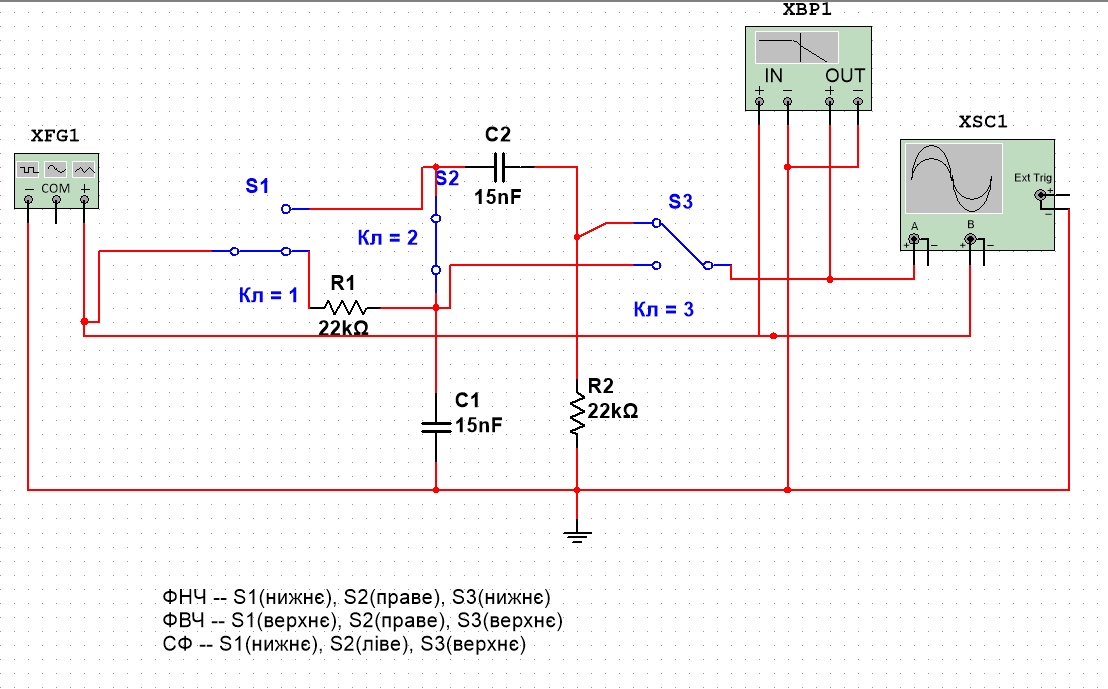
\includegraphics[width=.6\textwidth]{imgs/SF-1.png}
  \caption{Схема СФ}
\end{figure}
\begin{figure}[H]
  \centering
  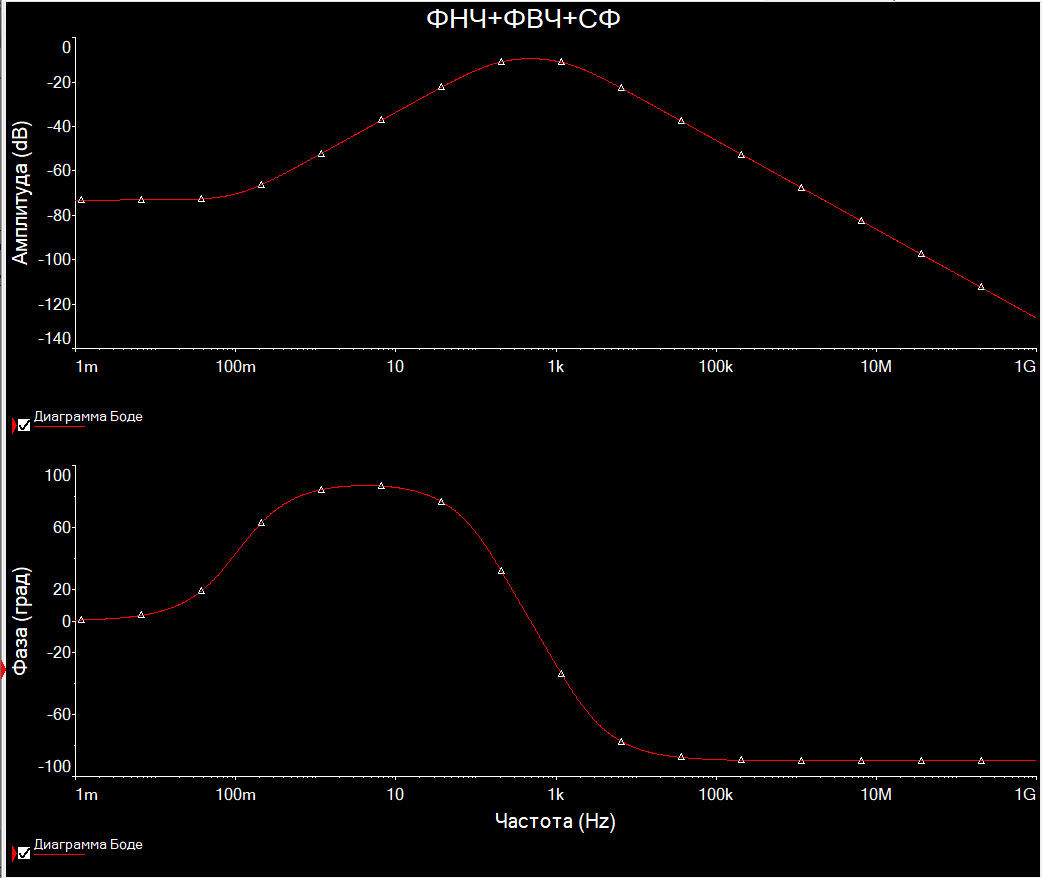
\includegraphics[width=.6\textwidth]{imgs/SF-2.png}
  \caption{Частотна характеристика}
\end{figure}
\begin{figure}[H]
  \centering
  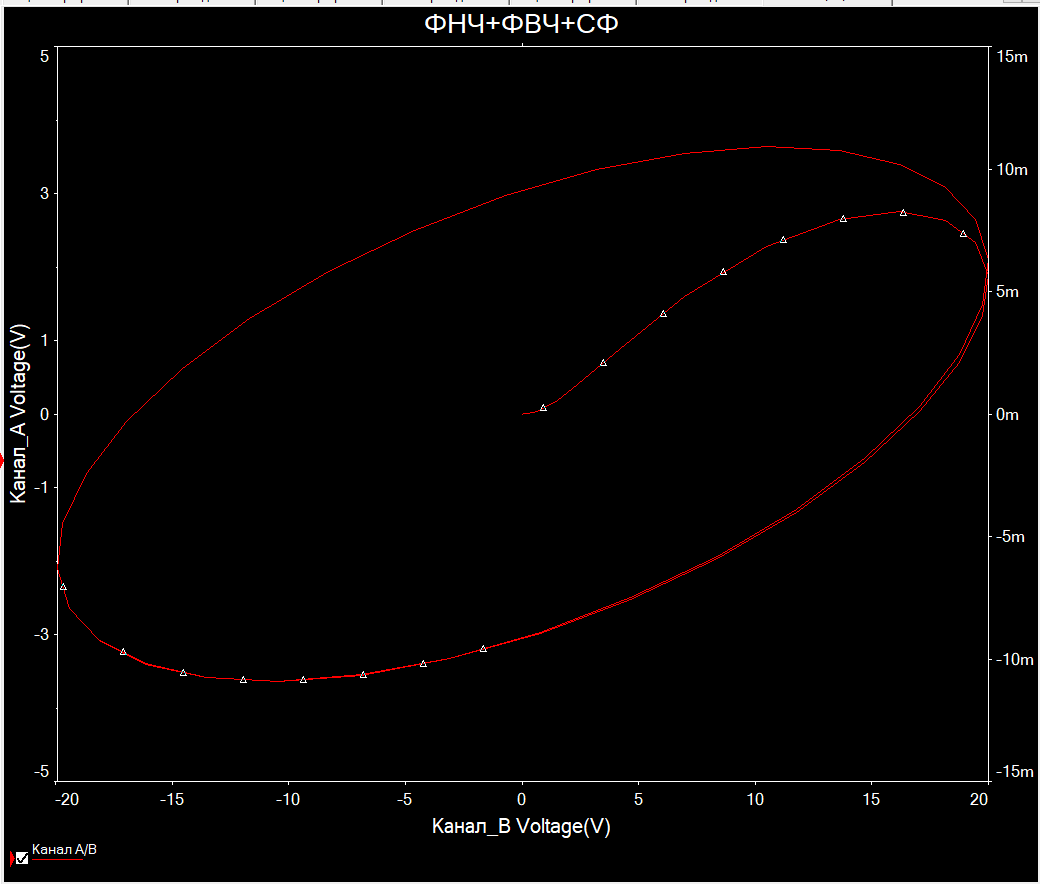
\includegraphics[width=.6\textwidth]{imgs/SF-3.png}
  \caption{Фігура Лісажу}
\end{figure}
\begin{figure}[H]
  \centering
  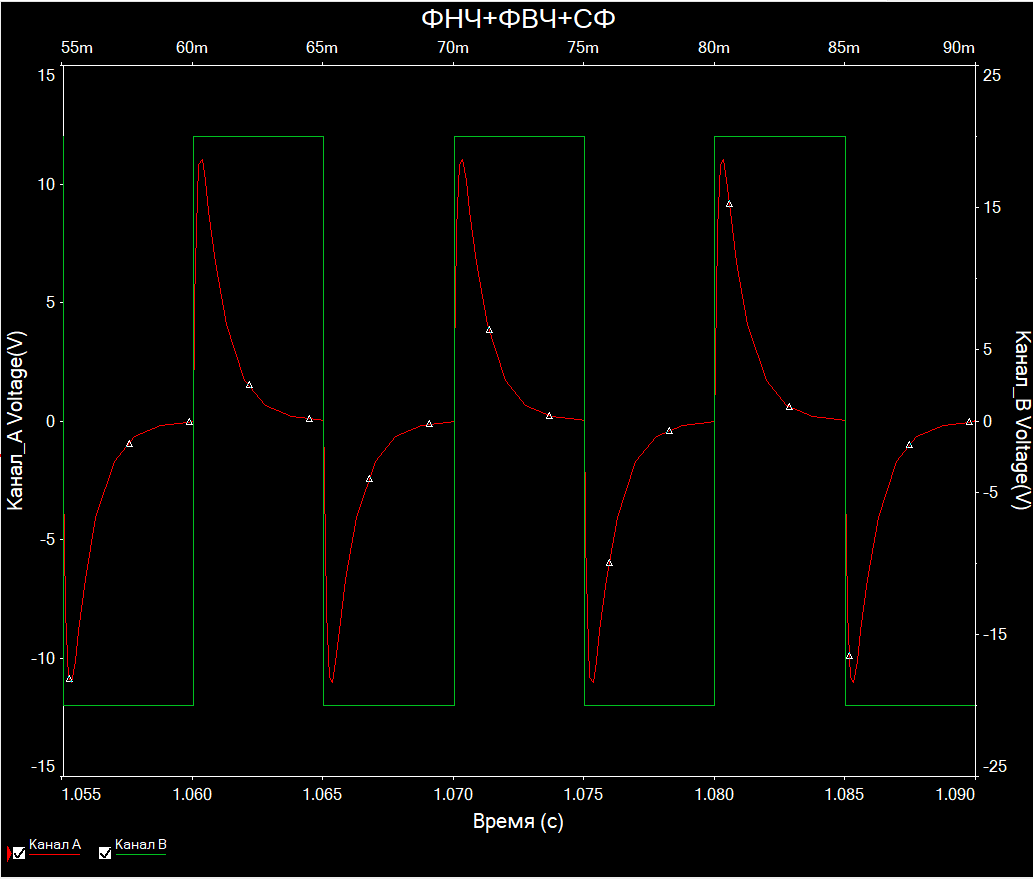
\includegraphics[width=.6\textwidth]{imgs/SF-4.png}
  \caption{Реакція на дискретний сигнал}
\end{figure}

\subsection{Загороджувальний фільтр}
\begin{figure}[H]
  \centering
  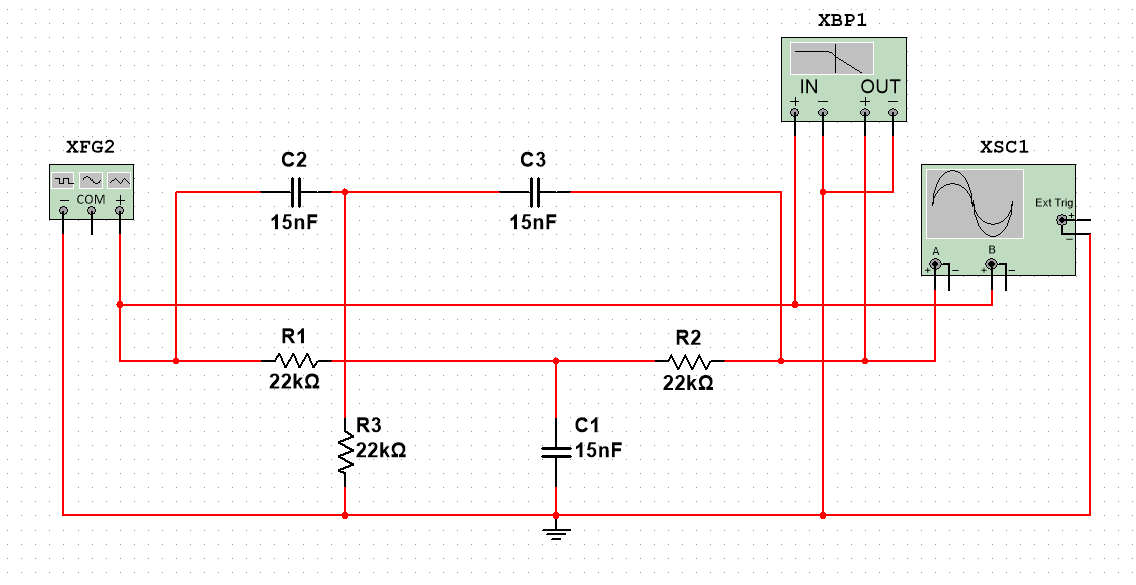
\includegraphics[width=.6\textwidth]{imgs/ZF-1.png}
  \caption{Схема ЗФ}
\end{figure}
\begin{figure}[H]
  \centering
  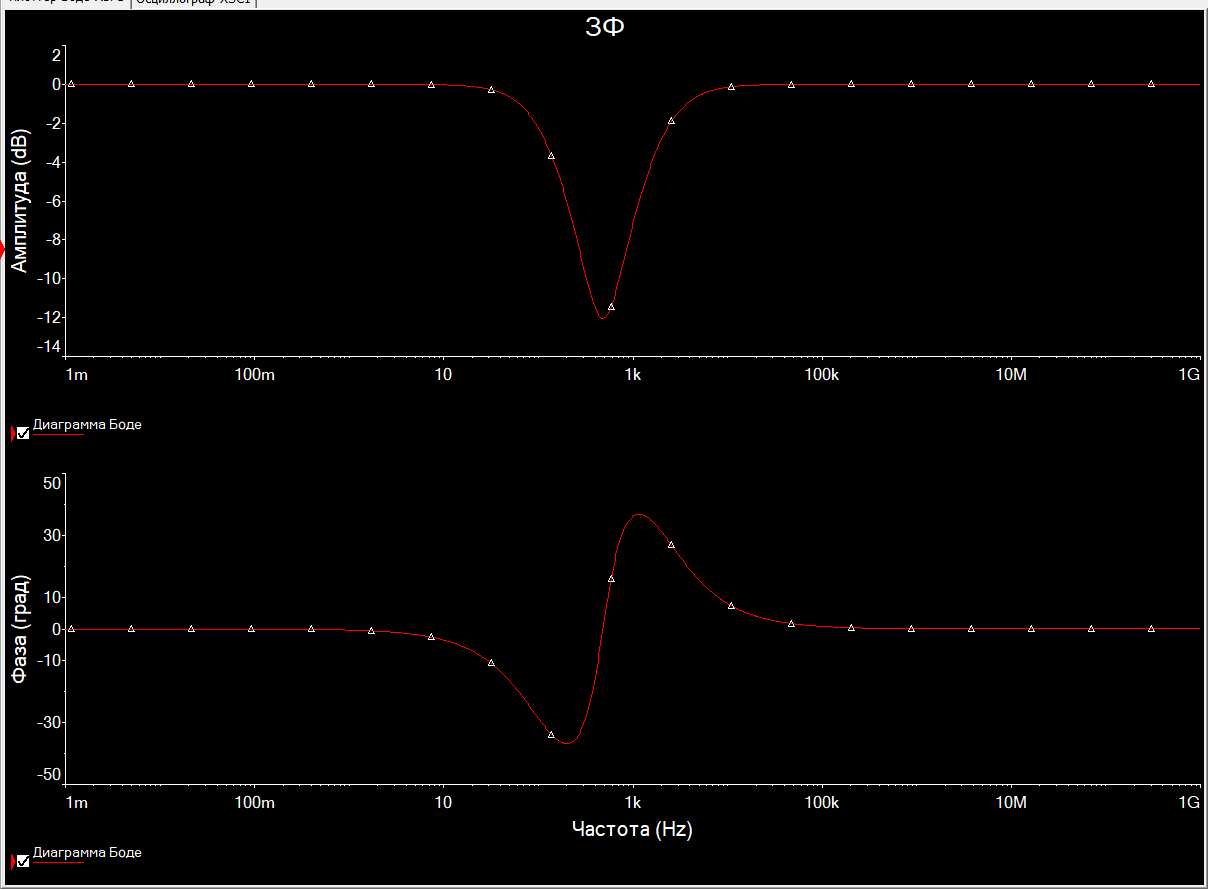
\includegraphics[width=.6\textwidth]{imgs/ZF-2.png}
  \caption{Частотна характеристика}
\end{figure}
\begin{figure}[H]
  \centering
  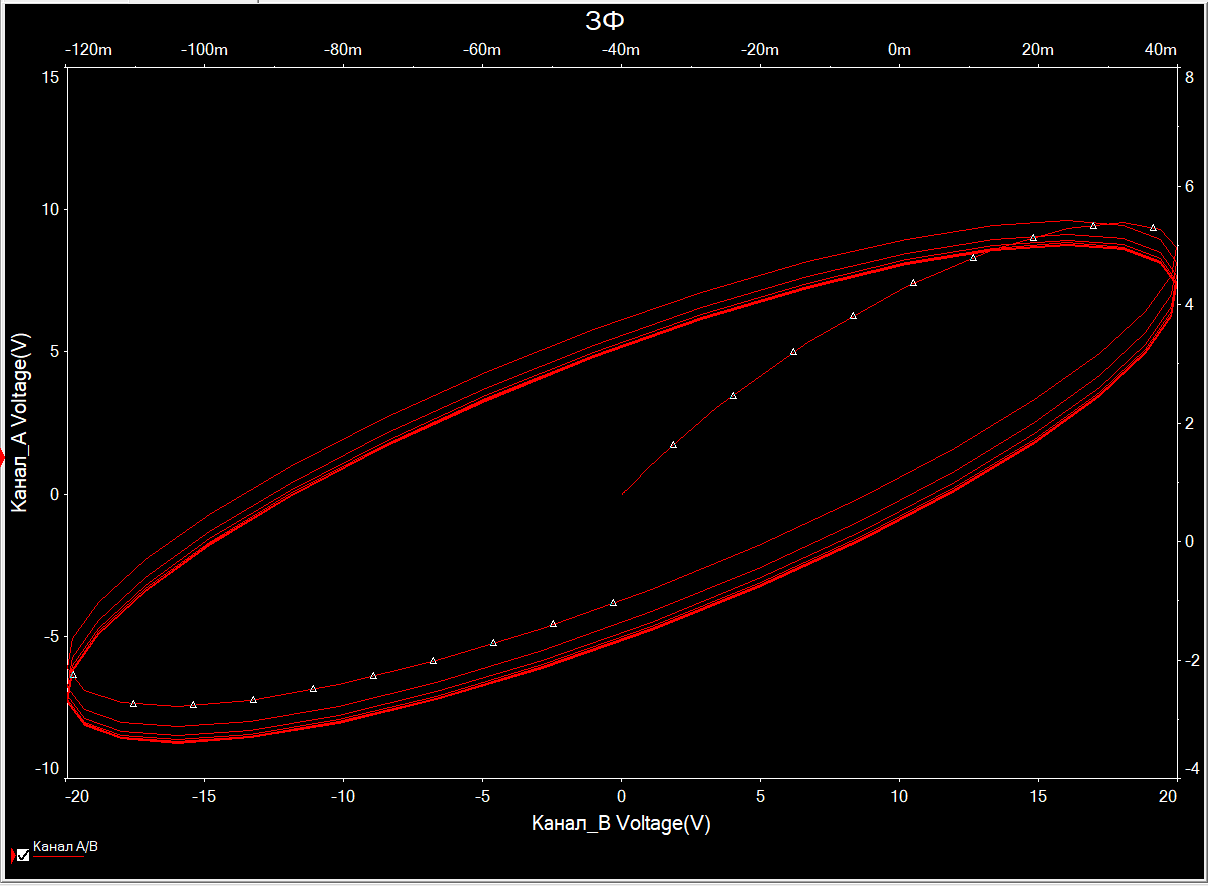
\includegraphics[width=.6\textwidth]{imgs/ZF-3.png}
  \caption{Фігура Лісажу}
\end{figure}
\begin{figure}[H]
  \centering
  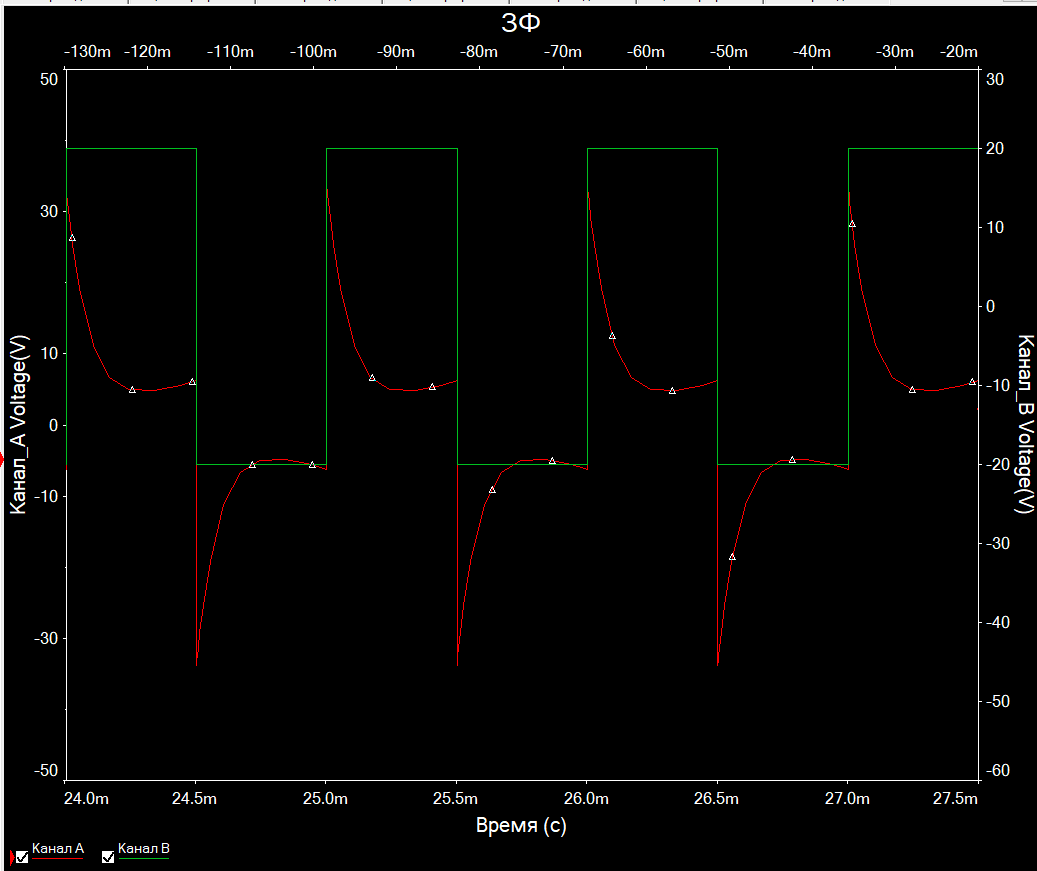
\includegraphics[width=.6\textwidth]{imgs/ZF-4.png}
  \caption{Реакція на дискретний сигнал}
\end{figure}

\section{Висновок}
У даній лабораторній роботі ми дослідили зміну
параметрів сигналів при їх проходженні через пасивні лінійні чотириполюсники. В дослідженні використовувалось два типи вхідних сигналів: гармонічні
(синусоїдальні) та прямокутні імпульси. Було вивчено також амплітудно-фазові
частотні характристики пасивних RC-фільтрів. Використано методи:
\begin{itemize}
  \item фігур Лісажу, який полягає у спостереженні на екрані двоканального осцило-
  графа замкнених кривих, які є результатом накладання двох коливань, що відбуваються
  у двох взаємно перпендикулярних напрямках (вхідний і вихідний сигнали подаються на
  пластини горизонтального та вертикального відхилення осцилографа відповідно). Як
  результат, дослідили і наочно переконалися в принципах проботи ФВЧ, ФНЧ та заго-
  роджувального фільтра, спостерігаючи проходження крізь них лише виділеної частини
  сигналу.
  \item співставлення, тобто одночасного спостереження вхідного та вихідного си-
  гналів на екрані двоканального осцилографа із наступним вимірюванням і порівнянням
  їх параметрів;
\end{itemize}

Робота виконувалась у програмі \textbf{Multisim14}.
\end{document}